\newpage

\section{Gateway module hardware}

The gateway module is designed as a Raspberry Pi HAT board. It has to contain
necessary hardware for power regulation and car communication. It also has to expose
all IO for connecting external devices such as an ESP32 programmer and a power cable
for the Raspberry Pi display.

\subsection{Communication hardware}
In section \ref{sec:van_bus} we have established that the VAN bus is a differential
protocol much like the CAN bus and, as a result, we can use readily available CAN
transciever hardware. However, we still need hardware that can generate valid VAN
frames. For that we use the Atmel TSS463C VAN driver chip. It is the only VAN driver chip
that exists. For the CAN transciever we use the MCP2551 because it was proven to work with 
early prototypes and, with it's 5 volt logic, integrates nicely with the TSS.

\begin{figure}[H]
    \begin{minipage}{0.48\textwidth}
        \begin{center}
            
\includegraphics[width=\textwidth]{images/sch_tss.pdf}
        \end{center}
    \end{minipage}
    \hfill\vline\hfill
    \begin{minipage}{0.48\textwidth}
        \begin{center}
            
\includegraphics[width=\textwidth]{images/sch_mcp.pdf}
        \end{center}
    \end{minipage}
    \caption{TSS463C and MCP2551 in the schematic}
\end{figure}
    

\subsubsection{TSS463C}

The TSS463C is the VAN driver chip we use for sending VAN frames to the car. It is the only
standalone VAN driver chip that exists, as all other modules inside the car have a VAN driver
built into their SOCs. The TSS uses SPI to communicate with the ESP32.

\subsection{Voltage levels}

The TSS463C and the MCP2551 both use 5V logic, while all other components on the board, including
the ESP32, use 3.3V logic. For that we use a pair of NTS0104 level shifters. One of them is used
for the TSS SPI communication with the ESP, while the other is used for connecting the VAN RX line
from the MCP to the ESP32 for reading VAN frames, and the TSS interrupt pin.

\subsection{Connecting to the car}

We are connecting to the car in place of the CD Changer unit. The CD Changer connects to
the original RD3 Headunit in the C3 (pins 13 to 20) portion of the ISO 10487 radio connector.
See Figure \ref{fig:iso-conn-pinout} for the pinout.

\bigskip
\noindent
Pins 13 to 17 for data and power are connected to the gateway module with a JST GH 6 pin connector,
while pins 18 to 20 are wired to a 3.5mm audio cable and connected to the Raspberry Pi. Since the
naming convention is different between Figures \ref{fig:iso-conn-pinout} and \ref{fig:jst-van-pinout},
see

\begin{minipage}{0.45\textwidth}
    \begin{figure}[H]
        \begin{center}
            
\includegraphics[width=\textwidth]{images/ISO-conn.pdf}
            \caption{ISO connector pinout}
            \label{fig:iso-conn-pinout}
        \end{center}
    \end{figure}    
\end{minipage}
\hfill\vline\hfill
\begin{minipage}{0.45\textwidth}
    \begin{figure}[H]
        \begin{center}
            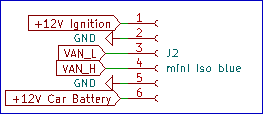
\includegraphics[width=\textwidth]{images/sch-jst-van.pdf}
            \caption{JST Connector in the schematic}
            \label{fig:jst-van-pinout}
        \end{center}
    \end{figure}  
\end{minipage}

\begin{table}[H]
    \begin{center}
        \begin{tabular}{|r c l|}
            \hline
            \texttt{VAN DATA} & $\Leftrightarrow$ & \texttt{VAN\_L} \\
            \hline
            \texttt{VAN DATA/} & $\Leftrightarrow$ & \texttt{VAN\_H} \\
            \hline
            \texttt{CD A/C GND} & $\Leftrightarrow$ & \texttt{GND} \\
            \hline
            \texttt{CD A/C B/U} & $\Leftrightarrow$ & \texttt{+12V Car Battery} \\
            \hline
            \texttt{+VAN} & $\Leftrightarrow$ & \texttt{+12V Ignition} \\
            \hline
        \end{tabular}
    \end{center}
    \caption{ISO to JST connection legend}
\end{table}

\subsection{ESP32 Flashing}

Flashing firmware on the ESP32 is done using UART. In order to flash the firmware, the
ESP must first be put into flashing mode. This can be done by pulling pins \texttt{GPIO00}
and \texttt{GPIO02} low when powering on the board. This can be achived in two ways
on our board: Manually by pressing the \texttt{BOOT} momentary button while resetting the
board with the \texttt{EN} button, or by connecting the \texttt{DTR} and \texttt{RTS} signals
of the UART adapter to the apropriate pins on the JST programming connector. They are 
connected internally to the \texttt{EN} and \texttt{GPIO00} inputs and the ESP programmer
(\texttt{esptool.py}) supports resetting and flashing the board using those signals.

\bigskip
\noindent
The UART programming interface is exposed on another JST GH 6 pin connector as well as
the \texttt{DTR} and \texttt{RTS} signals.

\begin{minipage}{0.45\textwidth}
    \begin{figure}[H]
        \begin{center}
            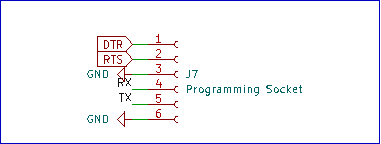
\includegraphics[width=\textwidth]{images/sch-prog-header.pdf}
        \end{center}
        \caption{Programming header pinout}
    \end{figure}
\end{minipage}
\hfill\vline\hfill
\begin{minipage}{0.45\textwidth}
    \begin{figure}[H]
        \begin{center}
            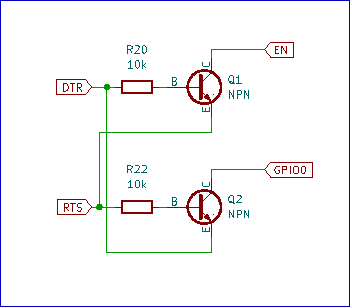
\includegraphics[width=\textwidth]{images/sch-prog-npn.pdf}
        \end{center}
        \caption{DTR and RTS signals}
    \end{figure}
\end{minipage}

\subsection{Power}

For power, we have two 12V voltage rails to work with. The first one is always live (\texttt{+12V Car Battery}), and the second one is switched on only when the car is awake (\texttt{+12V Ignition}).
The second rail is incorrectly labeled as it doesn't exactly follow the ignition key state, but the car's awake state. The car
will wake up when an action happens (locks lock/unlock, doors open/close, key gets put in the ACC position, etc.) and will go to sleep after some
time if nothing is happening and the key is not in the ACC position.

\bigskip
\noindent
As we have two rails, we have two separate voltage regulators (MP8759GD1) tasked with turning the 12 V from the input into 5 V at the output. 
The voltage regulator on the \texttt{+12V battery} rail is used to power the ESP32, TSS, and MCP chips, as they need to be able to be active even when the car is in sleep mode. 
However, as the ESP32 requires 3.3 V, we had to expand the design with a single 3.3V LDO voltage regulator.

\bigskip
\noindent
The other 5 V voltage regulator is tasked with supplying the RPi and the peripheral LCD with power. 
As they are not used for communicating with the car, there is no need for them to have a constant power supply.

\bigskip
\noindent
Apart from the voltage regulator ICs, on the schematic there is an outstanding number of filtering capacitors. 
They are required to provide a stable voltage source for the other ICs, as some of them are quite sensitive to noise and could start behaving in unexpected ways.
Another, often overlooked component when designing power supplies is the TVS diode, 
which is connected to the regulator input in a reverse polarized configuration, ensuring a maximum voltage of 12 V.

\subsection{Raspberry Pi}

The RPi is a slave to the ESP32 in the sense that it does not handle any communication with the car or any other system-critical matter. 
Its job is to render the telemetry data received from the ESP32 over UART on the LCD and handle the \emph{entertainment} part of the infotainment system. 
As a noncritical part of the system, there is no need for uninterrupted power access; hence, it is powered only when the car is awake according
to table \ref{tbl:car-states}.

\subsection{Misc}

\paragraph{RTC}
As the existing car display doesn't report the time on the bus, an additional RTC was needed. The selected RTC is DS3231MZ.
It's connected to the Raspberry Pi over I2C. It is readily available, accurate and supported out of the box by the Linux kernel.

\bigskip
\noindent
In order to be able to read out the battery voltage with the ESP32 ADCs, a simple resistor voltage divider circuit was used. 
With a division ratio of 4:1, on pin 9, IO33, there is 1/5 of the battery voltage. 
The resistors are in the 100 k$\Omega$ range, ensuring a current in the 10 $\mu$A range.

\bigskip
\noindent
To help with debugging, there are many LEDs placed on the communication and power lines along with a few debug connectors.

\subsection{Design defects}

Of course, a project isn't proper if everything works the first time. The PCB has a couple design defects that were able to
be bypassed. We will outline some of them here.

\paragraph{Strapping pins}

We made a mistake and overlooked some ESP32 strapping pins. They are pins used by the ESP during boot to set some parameters.
The pin we overlooked was GPIO12. This pin sets the voltage level of the internal SPI flash on which the firmware is stored.
This pin is shared by the SPI bus used to communicate with the TSS, and as a result the state of the pin was always undetermined.
This resulted in the board having issues booting and flashing sometimes. It was bypassed by burning an eFuse to set the
voltage level permanently.

\paragraph{MCP and TSS reset pins}

The MCP2551 can be put into a low power state by the Rs pin. We had the idea of controlling the state of that pin using
a transistor switch. However, the switch was incorrectly designed and the MCP was always in a low power state. This prevented
us from transmitting data to the VAN bus. This was bypassed by permanently putting the MCP into a running state with a 10k$\Omega$
pulldown. This resulted in increased idle power consumption by a few mA.

\bigskip
\noindent
The same issue was with the reset pin on the TSS463C. However, the TSS is always reset by software on boot, so that was easily bypassed
by just removing all components around the reset pin.

\paragraph{Level shifter}

The level shifter used for the VAN RX line connected to the ESP32 used the \texttt{+5V Ignition} rail as the reference for
the 5V side. This rail, however, was turned off when the ESP decided the Raspberry Pi shouldn't be powered on. As a result,
the ESP would power this down and never receive a VAN frame again, preventing the firmware from powering the rail back on.
This was bypassed by cutting the trace and connecting the reference to the \texttt{+5V Battery} rail.